\documentclass{beamer}

\usetheme{McMaster}
\usepackage{math}

%===Specific for this talk===%
\usepackage{algorithm,algorithmicx,algpseudocode}
\DeclareMathOperator{\iaa}{IAA} % paper specific
\newtheorem{proposition}{Proposition}
\newcommand{\vecw}{\left ( \vec{w}_i^n \right )^\top}
\newcommand{\Aij}{\left ( \hat{A} + E_{i \to j}^{n} \right )^{-1}}
\newcommand{\AijE}{\Aij E_{i \to j}^{n}}
\DeclareMathOperator{\Span}{span}

\title{Adaptive optimized Schwarz methods}
\author{Conor McCoid}
\institute{McMaster University}
\date{January 24th, 2025}

\begin{document}

\maketitle

\section{Brief history of domain decomposition} % 5 min

% Schwarz (incl. keyhole domain)

% P.L. Lions

% OSM? incl. algebraic transmission conditions

% ASPIN/MSPIN/RASPEN

\section{Alternate minimization in phase-field fracture models} % 15 min

% phase-field fracture model

% algebraic form of equations

% alternate minimization

% AltMin as multiplicative Schwarz

% applying Newton -> MSPIN

\section{Adaptive optimized Schwarz methods} % 30 min

% predictor-corrector formulation
\begin{frame}{Schwarz method with adaptive transmission conditions}

Let $T_{i \to j}$ change at each iteration, so that the transmission conditions adapt.
We can formulate such a Schwarz method, acting only on the difference in successive solutions,n as
\begin{equation*}
	\begin{bmatrix} A_{ii} & A_{i \Gamma} \\ A_{\Gamma i} & A_{\Gamma \Gamma} + T_{j \to i}^{n+1} \end{bmatrix}
	\begin{bmatrix} \vec{d}_i^{n+1} \\ \vec{d}_{i \Gamma}^{n+1} \end{bmatrix}
	= \begin{bmatrix} ~ \\ -A_{\Gamma j} \vec{d}_j^n + T_{j \to i}^{n+1} \vec{d}_{j \Gamma}^n - \Delta T_{j \to i}^n \left ( \vec{u}_{i \Gamma}^n - \vec{u}_{j \Gamma}^{n-1} \right ) \end{bmatrix},
\end{equation*}
where $i=1,2$, $j=3-i$, and $\Delta T_{j \to i}^n$ represents the update to the transmission condition $T_{j \to i}^n$ at this step,
\begin{equation*}
	T_{j \to i}^{n+1} = T_{j \to i}^n + \Delta T_{j \to i}^n.
\end{equation*}
\end{frame}

\begin{frame}{Condensing the iteration}

We can condense these iterations to express them as only acting on the difference at the interface.
First we note from the first row of blocks that
\begin{equation*}
	\vec{d}_i^{n+1} = -A_{ii}^{-1} A_{i \Gamma} \vec{d}_{i \Gamma}^{n+1},
\end{equation*}
and so likewise
\begin{equation*}
	\vec{d}_j^{n} = -A_{jj}^{-1} A_{j \Gamma} \vec{d}_{j \Gamma}^{n}.
\end{equation*}
Combining with the second row of blocks gives
\begin{align*}
	\left ( A_{\Gamma \Gamma} + S_{i \to j} + T_{j \to i}^{n+1} \right ) \vec{d}_{i \Gamma}^{n+1} =
	& \left ( T_{j \to i}^{n+1} - S_{j \to i} \right ) \vec{d}_{j \Gamma}^n \\
	& - \Delta T_{j \to i}^n \left ( \vec{u}_{i \Gamma} - \vec{u}_{j \Gamma}^{n-1} \right ).
\end{align*}
\end{frame}

\begin{frame}{Difference between $T$ and $S$}
Notice the difference between the $T$ matrices and the Schur complements in these systems.
If we represent this difference as
\begin{equation*}
	E_{i \to j}^{n+1} := T_{i \to j}^{n+1} - S_{i \to j},
\end{equation*}
and write $\hat{A} := A_{\Gamma \Gamma} + S_{1 \to 2} + S_{2 \to 1}$, then these systems become
\begin{equation*}
	\left ( \hat{A} + E_{i \to j}^{n+1} \right ) \vec{d}_{j \Gamma}^{n+1} = E_{i \to j}^{n+1} \vec{d}_{i \Gamma}^n - \Delta T_{i \to j}^n \left ( \vec{u}_{j \Gamma}^n - \vec{u}_{i \Gamma}^{n-1} \right ).
\end{equation*}
The matrix $E_{i \to j}^{n+1}$ is as expensive to calculate as the Schur complement, meaning this system is not practical.
However, it has immense theoretical value.
\end{frame}

\begin{frame}{Action of $E$}
The matrix-vector product $E_{i \to j}^{n+1} \vec{d}_{i \Gamma}^n$, equal to
\begin{equation*}
	E_{i \to j}^{n+1} \vec{d}_{i \Gamma}^n = -A_{\Gamma i} \vec{d}_i^n + T_{i \to j}^{n+1} \vec{d}_{i \Gamma}^n,
\end{equation*}
is computed in the course of the Schwarz method.
Thus, we will have a sequence of vector pairs, $\left ( \vec{d}_{i \Gamma}^n, E_{i \to j}^{n+1} \vec{d}_{i \Gamma}^n \right )$ which we can use to approximate $E$ without ever calculating it.

Each vector pair gives a rank one approximation of $E$:
\begin{equation*}
	E_{i \to j}^{n+1} \approx \frac{E_{i \to j}^{n+1} \vec{d}_{i \Gamma}^n}{\norm{\vec{d}_{i \Gamma}^n}_2^2}.
\end{equation*}
To combine these rank one matrices, we apply \textbf{modified Gram-Schmidt} to the vectors $\vec{d}$ and a commenserate process to the vectors $E \vec{d}$.
\end{frame}

% IAA algo + lemma
\begin{frame}
\begin{algorithm}[H]
	\caption{Iterative action approximation \\ $[V_n,W_n]=\iaa \left ( \set{\vec{x}_k}_{k=1}^n, E \right )$}
	\begin{algorithmic}[1]
		\State Inputs: $\set{\vec{x}_k}_{k=1}^{n} \subset \bbr^M$, $E \in \bbr^{M \times M}$
		\State $\alpha_1 := 1 / \norm{\vec{x}_1}$, $\vec{w}_1 := \alpha_1 \vec{x}_1$, $\vec{v}_1 := \alpha_1 E \vec{x}_1$
		\For{$k=2 : n$}
			\State $\vec{w}_k := \vec{x}_k$, $\vec{v}_k := E \vec{x}_k$
			\For{$i=1 : k-1$}
				\State $h \gets \langle \vec{w}_i, \vec{w}_k \rangle$, $\vec{w}_k \gets \vec{w}_k - h \vec{w}_i$
				\State $\vec{v}_k \gets \vec{v}_k - h \vec{v}_i$ \label{line: implicit}
			\EndFor
			\State $\alpha_k := 1 / \norm{\vec{w}_k}$, $\vec{w}_k \gets \alpha_k \vec{w}_k$, $\vec{v}_k \gets \alpha_k \vec{v}_k$
		\EndFor
		\State Outputs: $W_{n} = \begin{bmatrix} \vec{w}_1 & \vec{w}_2 & \dots & \vec{w}_{n} \end{bmatrix}$, $V_{n} = \begin{bmatrix} \vec{v}_1 & \vec{v}_2 & \dots & \vec{v}_{n} \end{bmatrix}$
		\State $V_{n} W_{n}^\top \approx E$
	\end{algorithmic}
	\label{alg: IAA}
\end{algorithm}
\end{frame}

\begin{frame}{Properties of the IAA}
\begin{lemma} \label{lem: iaa}
	Let $\mathcal{S}=\set{\vec{x}_k}_{k=1}^n \subset \bbr^M$ be a set of linearly independent vectors, $E \in \bbr^{M \times M}$ a matrix.
	Let $[V_n,W_n]=\iaa(\mathcal{S},E)$ with columns $\vec{v}_k$ and $\vec{w}_k$, respectively.
	Let $E^1 := E$ and let $E^{k+1} := E^k - \vec{v}_k \vec{w}_k^\top$.
	Then
	\begin{align*}
		E^{k+1} = & E (I - W_k W_k^\top), \\
		\vec{v}_k = & E \vec{w}_k = E^k \vec{w}_k
	\end{align*}
	for $1 \leq k \leq n$, where $W_k$ is the first $k$ columns of $W_n$.
\end{lemma}
\end{frame}

% choice of adaptive transmission conditions + altAOSM + solve ladder(s?)
\begin{frame}{Choice of adaptive transmission conditions}
For our adaptive transmission conditions, we want
\begin{align*}
	[ V_i^n, W_i^n ] & = \iaa \left ( \set{ \vec{d}_{i \Gamma}^k }_{k=1}^n, E_{i \to j}^1 \right ), \\
	\text{where} \ E_{i \to j}^1 \vec{d}_{i \Gamma}^k & = -A_{\Gamma i} \vec{d}_i^k + T_{i \to j}^1 \vec{d}_{i \Gamma}^k.
\end{align*}
Each time we find a new $\vec{d}_{i \Gamma}^k$, with corresponding $\vec{d}_i^k$, we can compute a new $\vec{v}_i^k$ and $\vec{w}_i^k$.
This gives us a rank one update to the transmission conditions:
\begin{equation*}
	\Delta T_{i \to j}^n = - \vec{v}_i^k \left ( \vec{w}_i^k \right )^\top.
\end{equation*}

This choice of $\Delta T$ eliminates the product $E_{i \to j}^{n+1} \vec{d}_{i \Gamma}^n$ from the earlier systems.
We must now solve
\begin{equation*}
	\begin{bmatrix} A_{jj} & A_{j \Gamma} \\ A_{\Gamma j} & A_{\Gamma \Gamma} + T_{i \to j}^{n+1} \end{bmatrix}
	\begin{bmatrix} \vec{d}_j^{n+1} \\ \vec{d}_{j \Gamma}^{n+1} \end{bmatrix}
	= (\vec{w}_i^n)^\top \left ( \vec{u}_{j \Gamma}^n - \vec{u}_{i \Gamma}^{n-1} \right )\begin{bmatrix} ~ \\ \vec{v}_i^n \end{bmatrix}
\end{equation*}
at every step.
\end{frame}

\begin{frame}
\begin{algorithm}[H]
	\caption{altAOSM: AOSM applied to multiplicative Schwarz} %nb: include function defn like iaa?
	\label{alg: alt}
	\begin{algorithmic}[1]
		\State Start with initial transmission conditions $T_{1 \to 2}^1$ and $T_{2 \to 1}^1$
		\State Make initial guess $\vec{u}_{1 \Gamma}^0$
		\State Calculate $\vec{u}_1^0 = A_{11}^{-1} ( \vec{f}_1 - A_{1 \Gamma} \vec{u}_{1 \Gamma}^0 )$
		\State Solve for $\vec{u}_2^1$ and $\vec{u}_{2 \Gamma}^1$, then for $\vec{u}_1^2$ and $\vec{u}_{1 \Gamma}^2$
		\State Calculate $\vec{d}_{1 \Gamma}^2 = \vec{u}_{1 \Gamma}^2 - \vec{u}_{1 \Gamma}^0$ and $\vec{d}_1^2$ and set $n=2$
		\While{$\norm{ \vec{d}_{1 \Gamma}^n } + \norm{ \vec{d}_{2 \Gamma}^{n-1} } \geq tol$}
			\For{$i=1 : 2$}
				\State Run an iteration of IAA
				\State Set $\Delta T_{i \to j}^n = - \vec{v}_i^n (\vec{w}_i^n)^\top$
				\State Solve for $\vec{d}_{j \Gamma}^{n+1}$ and $\vec{d}_j^{n+1}$
				\State $\vec{u}_j^{n+1} := \vec{u}_j^{n-1} + \vec{d}_j^{n+1}$, $\vec{u}_{j \Gamma}^{n+1} := \vec{u}_{j \Gamma}^{n-1} + \vec{d}_{j \Gamma}^{n+1}$
				\State $n \gets n+1$
			\EndFor
		\EndWhile
		\State Output: $\vec{u} = [ \vec{u}_1^n \ ; \ (\vec{u}_{1 \Gamma}^n + \vec{u}_{2 \Gamma}^{n-1})/2 \ ; \ \vec{u}_2^{n-1} ]$
	\end{algorithmic}
\end{algorithm}
\end{frame}

\begin{frame}
\centering
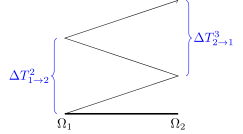
\includegraphics[width=0.45\textwidth]{AOSM/TIKZ_AOSM_20230614_3.png}
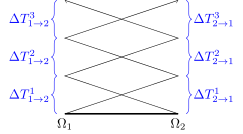
\includegraphics[width=0.45\textwidth]{AOSM/TIKZ_AOSM_20230614_4.png}
\end{frame}

% Galerkin condition for AOSM
\begin{frame}{AOSM Galerkin condition}

\begin{theorem} \label{thm: opt}
If $\hat{A} + E_{i \to j}^{n+1}$ is invertible, then the update to the solution due to an AOSM is $$\vec{d}_{j \Gamma}^{n+1} = \AijE \vec{x},$$ where
$\vec{x} \in  \Span(W_i^n)$ such that the residual of
\begin{align*}
	& \left ( I - \left ( \hat{A} + E_{i \to j}^{n+1} \right )^{-1} E_{i \to j}^{n+1} \right ) \vec{u}_\Gamma \\
	& = \left ( \hat{A} + E_{i \to j}^{n+1} \right )^{-1} \left ( \vec{f}_\Gamma - A_{\Gamma j} A_{jj}^{-1} \vec{f}_j - A_{\Gamma i} A_{ii}^{-1} \vec{f}_i \right )
\end{align*}
applied to $\vec{u}_{i \Gamma}^{n-1} + \vec{x}$ is orthogonal to $\Span(W_i^n)$. 
\end{theorem}
\end{frame}

% numerical results: basic comparison with GMRES

% multiple subdomains (Schur complements for red-black)

% symmetrized cells

\begin{frame}{Algebraic Schwarz}

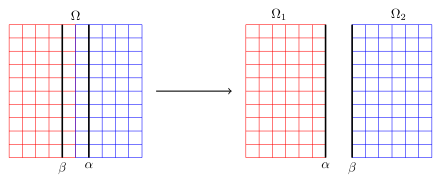
\includegraphics[width=\textwidth]{AOSM/TIKZ_AOSM_20230614_1.png}
\end{frame}

\begin{frame}{Algebraic Schwarz}
Consider the following algebraic system with block tridiagonal matrix $A$:
\begin{equation*}
	A \vec{u} = \begin{bmatrix} A_{11} & A_{1 \Gamma} \\ A_{\Gamma 2} & A_{\Gamma \Gamma} & A_{\Gamma 1} \\ ~ & A_{2 \Gamma} & A_{22} \end{bmatrix} \begin{bmatrix} \vec{u}_1 \\ \vec{u}_\Gamma \\ \vec{u}_2 \end{bmatrix} = \begin{bmatrix} \vec{f}_1 \\ \vec{f}_\Gamma \\ \vec{f}_2 \end{bmatrix} = \vec{f} .
\end{equation*}

The solution is divided into two subdomains: $\Omega_1$ contains the variables in $\vec{u}_1$ and $\vec{u}_\Gamma$, and $\Omega_2$ contains the variables in $\vec{u}_2$ and $\vec{u}_\Gamma$.
The variables $\vec{u}_\Gamma$ are then shared between the two subdomains.
We will refer to this portion as the \textbf{interface} between the two subdomains.

~

The idea is to find local solutions on each subdomain, a process which is easier to accomplish than solving the system as a whole.
To find a global solution, local solutions are found iteratively, with information on the interface passing between the two subdomains.
\end{frame}

\begin{frame}{Algebraic Schwarz}
There is a physical interpretation of this algebraic splitting, the more commonly seen Schwarz methods.
Consider the differential equation
\begin{equation*}
	\begin{cases} \Delta u(x,y) = f(x,y), & (x,y) \in \Omega = [-1,1] \times [-1,1], \\ u(x,y)=h(x,y), & (x,y) \in \partial \Omega. \end{cases}
\end{equation*}
Splitting this up using a Schwarz method results in the following subproblems that are solved iteratively:
\begin{align*}
	\begin{cases} \Delta u_1^n(x,y) = f(x,y), & (x,y) \in \Omega_1 = [-1,\alpha] \times [-1,1], \\ u_1^n(\alpha,y)=u_2^{n-1}(\alpha,y), \end{cases} \\
	\begin{cases} \Delta u_2^n(x,y) = f(x,y), & (x,y) \in \Omega_2 = [\beta,1] \times [-1,1], \\ u_2^n(\beta,y)=u_1^{n-1}(\beta,y). \end{cases}
\end{align*}
The \textbf{overlap}, physical equivalent of the interface, is now the region where $\beta \leq x \leq \alpha$.
Note that Dirichlet boundary conditions on this interface pass information between the subdomains.
\end{frame}

\begin{frame}{Algebraic Schwarz}
The two subdomains in algebraic Schwarz are
\begin{align*}
	\begin{bmatrix} A_{11} & A_{1 \Gamma} \\ A_{\Gamma 1} & A_{\Gamma \Gamma} + T_{2 \to 1} \end{bmatrix}
                            \begin{bmatrix} \vec{u}_1^{n+1} \\ \vec{u}_{1 \Gamma}^{n+1} \end{bmatrix}
                            = \begin{bmatrix} \vec{f}_1 \\ \vec{f}_\Gamma \end{bmatrix}
                            + \begin{bmatrix} ~ \\ -A_{\Gamma 2} \vec{u}_2^n + T_{2 \to 1} \vec{u}_{2 \Gamma}^n \end{bmatrix}, \\
       \begin{bmatrix} A_{22} & A_{2 \Gamma} \\ A_{\Gamma 2} & A_{\Gamma \Gamma} + T_{1 \to 2} \end{bmatrix}
                            \begin{bmatrix} \vec{u}_2^{n+1} \\ \vec{u}_{2 \Gamma}^{n+1} \end{bmatrix}
                            = \begin{bmatrix} \vec{f}_2 \\ \vec{f}_\Gamma \end{bmatrix}
                            + \begin{bmatrix} ~ \\ -A_{\Gamma 1} \vec{u}_1^n + T_{1 \to 2} \vec{u}_{1 \Gamma}^n \end{bmatrix} ,
\end{align*}
for any choice of matrices $T_{1 \to 2}$ and $T_{2 \to 1}$ (that does not make these systems singular).

~

Each choice of matrices $T$ corresponds to a choice of boundary conditions on the interface, called \textbf{transmission conditions}, since they transmit information between subdomains.
\end{frame}

\begin{frame}{Algebraic Schwarz}
For example, choosing $T=0$ is equivalent to Dirichlet transmission conditions (in most cases).
Note in this case, the Dirichlet information is taken from \textit{outside} the interface.

~

There is thus a disconnect between the physical overlap and the algebraic interface.
In fact, the same interface can represent both overlapping and non-overlapping subdomains, depending on $T$.

\centering
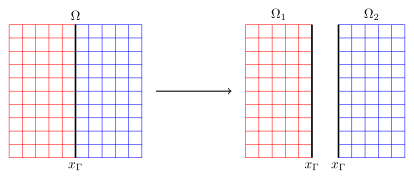
\includegraphics[width=0.7\textwidth]{AOSM/TIKZ_AOSM_20230614_2.png}
\end{frame}

\begin{frame}{Algebraic Schwarz}
Dirichlet transmission conditions generally provide slow convergence.
Optimized Schwarz methods use higher order transmission conditions with parameters to improve this convergence.
Easiest among these is Robin transmission conditions:
\begin{equation*}
	\frac{\partial u_1^n}{\partial x} - p u_1^n(0,y)= \frac{\partial u_2^{n-1}}{\partial x} - p u_2^{n-1}(0,y),
\end{equation*}
where one can find an optimal $p$.
This usually takes upfront Fourier analysis or similar methods, but produces significant speed-ups.

~

One can even go higher order, such as with tangential transmission conditions:
\begin{equation*}
	\frac{\partial u_1^n}{\partial x} - p u_1^n(0,y) + q \frac{\partial u_1^n}{\partial y}=
	\frac{\partial u_2^{n-1}}{\partial x} - p u_2^{n-1}(0,y) + q \frac{\partial u_2^n}{\partial y},
\end{equation*}
now giving parameters $p$ and $q$ to tweak.
\end{frame}

\begin{frame}{Algebraic Schwarz}
One can continue going to higher and higher order, with increasingly non-local information transmitted, until one has as many parameters to adjust as there are variables in the interface.
At the limit, one arrives at the optimal transmission conditions, \textbf{absorbing boundary conditions (ABCs)}, which are traditionally used to ensure incoming waves do not reflect at the boundary.
There are numerous methods for approximating ABCs, such as Pad\'e approximants and perfectly matched layers, each with their own benefits and drawbacks.

~

Algebraically, ABCs correspond to replacing the $T$ matrices with the Schur complements:
\begin{equation*}
	T_{i \to j} \to S_{i \to j} := -A_{\Gamma i} A_{ii}^{-1} A_{i \Gamma}.
\end{equation*}
With these, algebraic Schwarz with two subdomains converges in two iterations.
\end{frame}

\begin{frame}{Algebraic Schwarz}
Of course, if one has the Schur complements, algebraic Schwarz becomes a direct method.
But the Schur complements are expensive to calculate, and in general dense.
In the time it takes to calculate the Schur complements, one can run roughly the same number of subdomain solves as there are variables in the interface.

~

This puts an artificial limit on the number of iterations of algebraic Schwarz to run.
Let $M$ be the number of variables in the interface.
If algebraic Schwarz does not converge in $M$ iterations, we would have been better off computing the Schur complements.
\end{frame}

\begin{frame}{Adaptive Transmission Conditions}
We aim to construct black box approximations to these Schur complements / ABCs using vectors produced in the course of the algebraic Schwarz method.
These approximations will be updated at each iteration of the method.
The transmission conditions will then be \textbf{adaptive}.

~

This requires reformulating the original algebraic systems with fixed $T$ matrices to ones with adaptive $T$ matrices:
\begin{align*}
\begin{bmatrix} A_{11} & A_{1 \Gamma} \\ A_{\Gamma 1} & A_{\Gamma \Gamma} + T_{2 \to 1}^{n+1} \end{bmatrix}
\begin{bmatrix} \vec{u}_1^{n+1} \\ \vec{u}_{1 \Gamma}^{n+1} \end{bmatrix}
& = \begin{bmatrix} \vec{f}_1 \\ \vec{f}_\Gamma \end{bmatrix}
- \begin{bmatrix} ~ \\ A_{\Gamma 2} \vec{u}_2^n \end{bmatrix}
+ \begin{bmatrix} ~ \\ T_{2 \to 1}^{n+1} \vec{u}_{2 \Gamma}^n \end{bmatrix}, \\
\begin{bmatrix} A_{22} & A_{2 \Gamma} \\ A_{\Gamma 2} & A_{\Gamma \Gamma} + T_{1 \to 2}^{n+1} \end{bmatrix}
\begin{bmatrix} \vec{u}_2^{n+1} \\ \vec{u}_{2 \Gamma}^{n+1} \end{bmatrix}
& = \begin{bmatrix} \vec{f}_2 \\ \vec{f}_\Gamma \end{bmatrix}
- \begin{bmatrix} ~ \\ A_{\Gamma 1} \vec{u}_1^n \end{bmatrix}
+ \begin{bmatrix} ~ \\ T_{1 \to 2}^{n+1} \vec{u}_{1 \Gamma}^n \end{bmatrix}.
\end{align*}
Now $T_{i \to j}^{n+1}$ represents the transmission conditions used at step $n+1$.
\end{frame}

\begin{frame}{Adaptive Transmission Conditions}
How do we extract updates to the transmission conditions?
Let us reformulate the systems again, into a corrector form that works on the difference between successive iterates:
\begin{align*}
	& \begin{bmatrix} A_{11} & A_{1 \Gamma} \\ A_{\Gamma 1} & A_{\Gamma \Gamma} + T_{2 \to 1}^{n+1} \end{bmatrix}
	\left ( \begin{bmatrix} \vec{u}_1^{n+1} \\ \vec{u}_{1 \Gamma}^{n+1} \end{bmatrix} - \begin{bmatrix} \vec{u}_1^n \\ \vec{u}_{1 \Gamma}^n \end{bmatrix} \right ) \\
	& = \begin{bmatrix} A_{11} & A_{1 \Gamma} \\ A_{\Gamma 1} & A_{\Gamma \Gamma} + T_{2 \to 1}^{n+1} \end{bmatrix}
	\begin{bmatrix} \vec{u}_1^{n+1} \\ \vec{u}_{1 \Gamma}^{n+1} \end{bmatrix} \\
	& \quad - \begin{bmatrix} A_{11} & A_{1 \Gamma} \\ A_{\Gamma 1} & A_{\Gamma \Gamma} + T_{2 \to 1}^n \end{bmatrix}
	\begin{bmatrix} \vec{u}_1^n \\ \vec{u}_{1 \Gamma}^n \end{bmatrix}
	- \begin{bmatrix} ~ & ~ \\ ~ & \Delta T_{2 \to 1}^n \end{bmatrix} \begin{bmatrix} \vec{u}_1^n \\ \vec{u}_{1 \Gamma}^n \end{bmatrix} \\
	& = \begin{bmatrix} \vec{f}_1 \\ \vec{f}_\Gamma \end{bmatrix}
	- \begin{bmatrix} ~ \\ A_{\Gamma 2} \vec{u}_2^n \end{bmatrix}
	+ \begin{bmatrix} ~ \\ T_{2 \to 1}^{n+1} \vec{u}_{2 \Gamma}^n \end{bmatrix} \\
	& \quad - \left ( \begin{bmatrix} \vec{f}_1 \\ \vec{f}_\Gamma \end{bmatrix}
	- \begin{bmatrix} ~ \\ A_{\Gamma 2} \vec{u}_2^{n-1} \end{bmatrix}
	+ \begin{bmatrix} ~ \\ T_{2 \to 1}^n \vec{u}_{2 \Gamma}^{n-1} \end{bmatrix} \right )
	- \begin{bmatrix} ~ \\ \Delta T_{2 \to 1}^n \vec{u}_{1 \Gamma}^{n} \end{bmatrix},
\end{align*}
\end{frame}

\begin{frame}{Adaptive Transmission Conditions}
We focus on the matrix-vector product $E_{i \to j}^{n+1} \vec{d}_{i \Gamma}^n$.
Tracing backwards, this is equal to
\begin{equation*}
	E_{i \to j}^{n+1} \vec{d}_{i \Gamma}^n = -A_{\Gamma i} \vec{d}_i^n + T_{i \to j}^{n+1} \vec{d}_{i \Gamma}^n.
\end{equation*}
Thus, we can (and must) compute this matrix-vector product in the course of the method.

~

This gives us a sequence of vector pairs, $(\vec{d}_{i \Gamma}^n, E_{i \to j}^{n+1} \vec{d}_{i \Gamma}^n)$.
Let's use this sequence to construct an approximation to $E_{i \to j}^{n+1}$.
If we have an approximation to $E_{i \to j}^{n+1}$, we can subtract it from $T_{i \to j}^{n+1}$ to get an approximation of $S_{i \to j}^{n+1}$.
\end{frame}

\begin{frame}{Adaptive Transmission Conditions}
Let $\vec{y} = E \vec{d}$.
From one vector pair we can extract a rank one approximation of $E$:
\begin{equation*}
	E \approx \frac{\vec{y} \vec{d}^\top}{\norm{\vec{d}}_2^2}.
\end{equation*}
This approximation is only accurate when multiplying by vectors parallel to $\vec{d}$.

~

Each vector pair gives such a rank one approximation, but the sum of these approximations is only an approximation of $E$ if the vectors $\vec{d}$ are orthogonal, which is not true in general.
To fix this, we apply \textbf{modified Gram-Schmidt} to the set of vectors $\vec{d}$, resulting in the vectors $\vec{w}$.
To get the vectors $\vec{v}=E \vec{w}$, a commenserate process must be done on the vectors $\vec{y}$ (NOT MGS!).
\end{frame}

\begin{frame}{Numerical results}
\begin{equation*}
	\begin{cases} \Delta u(x,y) = f(x,y), & (x,y) \in \Omega = [-1,1] \times [-1,1], \\
		u(x,y) = g(x,y), & (x,y) \in \partial \Omega. % = \set{x=-1} \cup \set{x=1} \cup \set{y=-1} \cup \set{y=1} .
	\end{cases}
\end{equation*}
\begin{figure}
	\only<1>{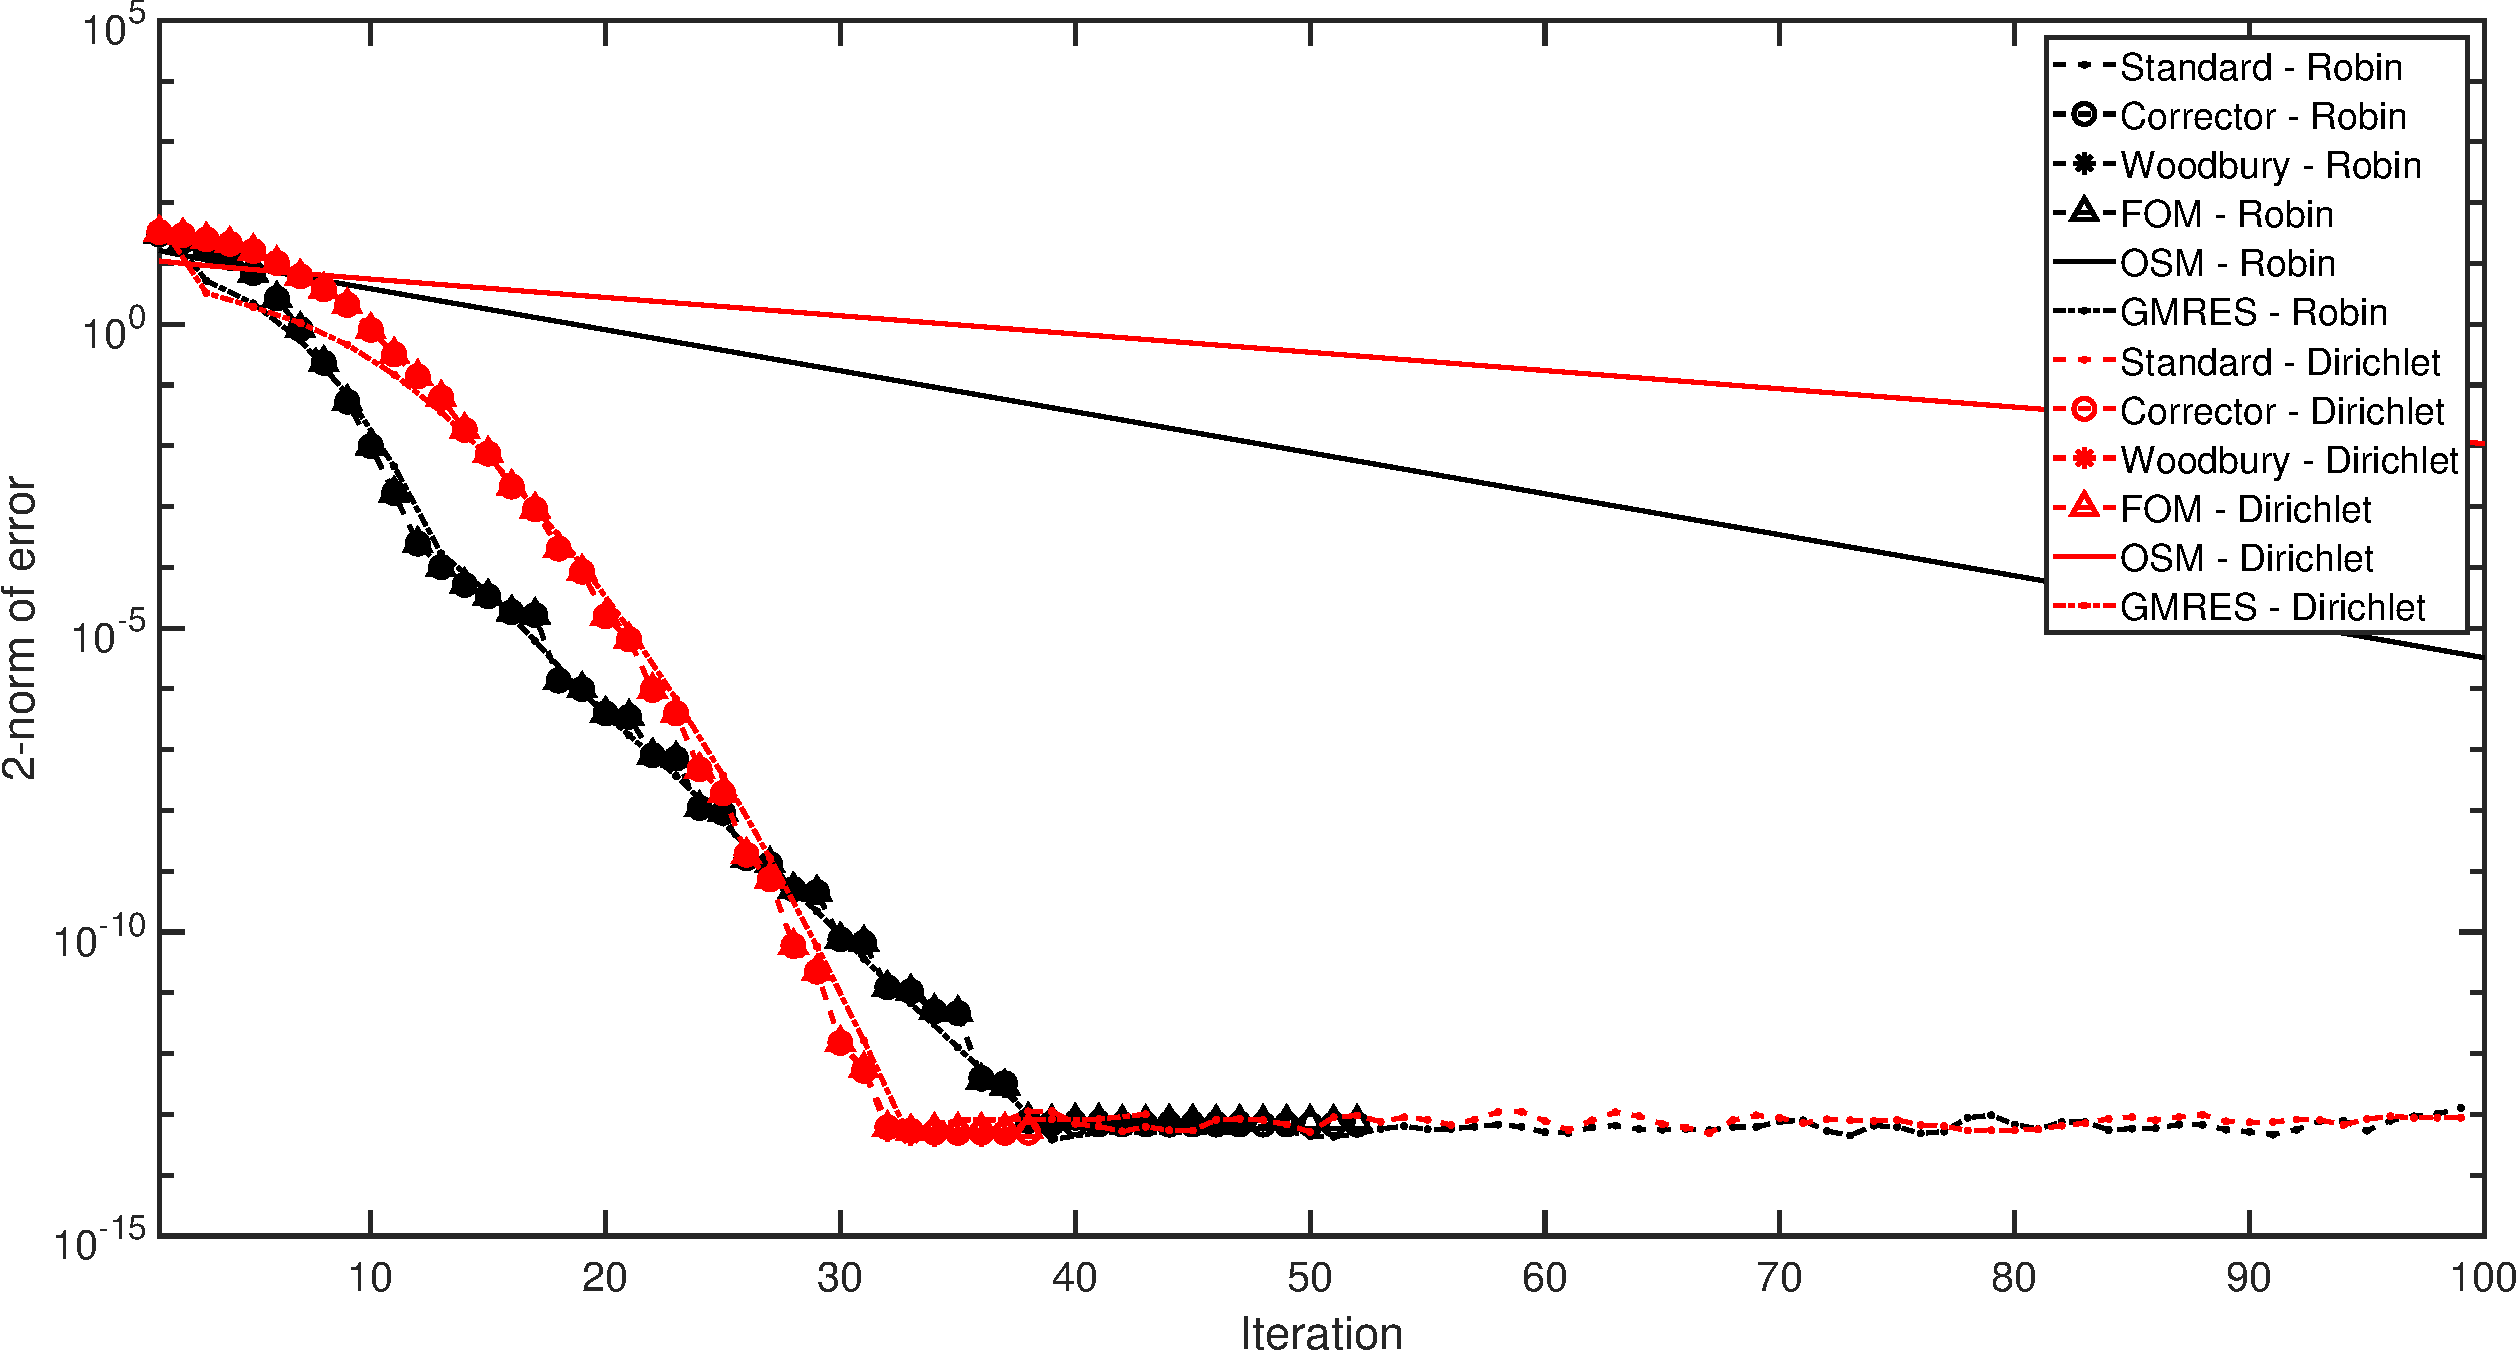
\includegraphics[width=0.75\textwidth]{AOSM/PLOT_faltAOSMConv_Laplace.pdf}}
	\only<2>{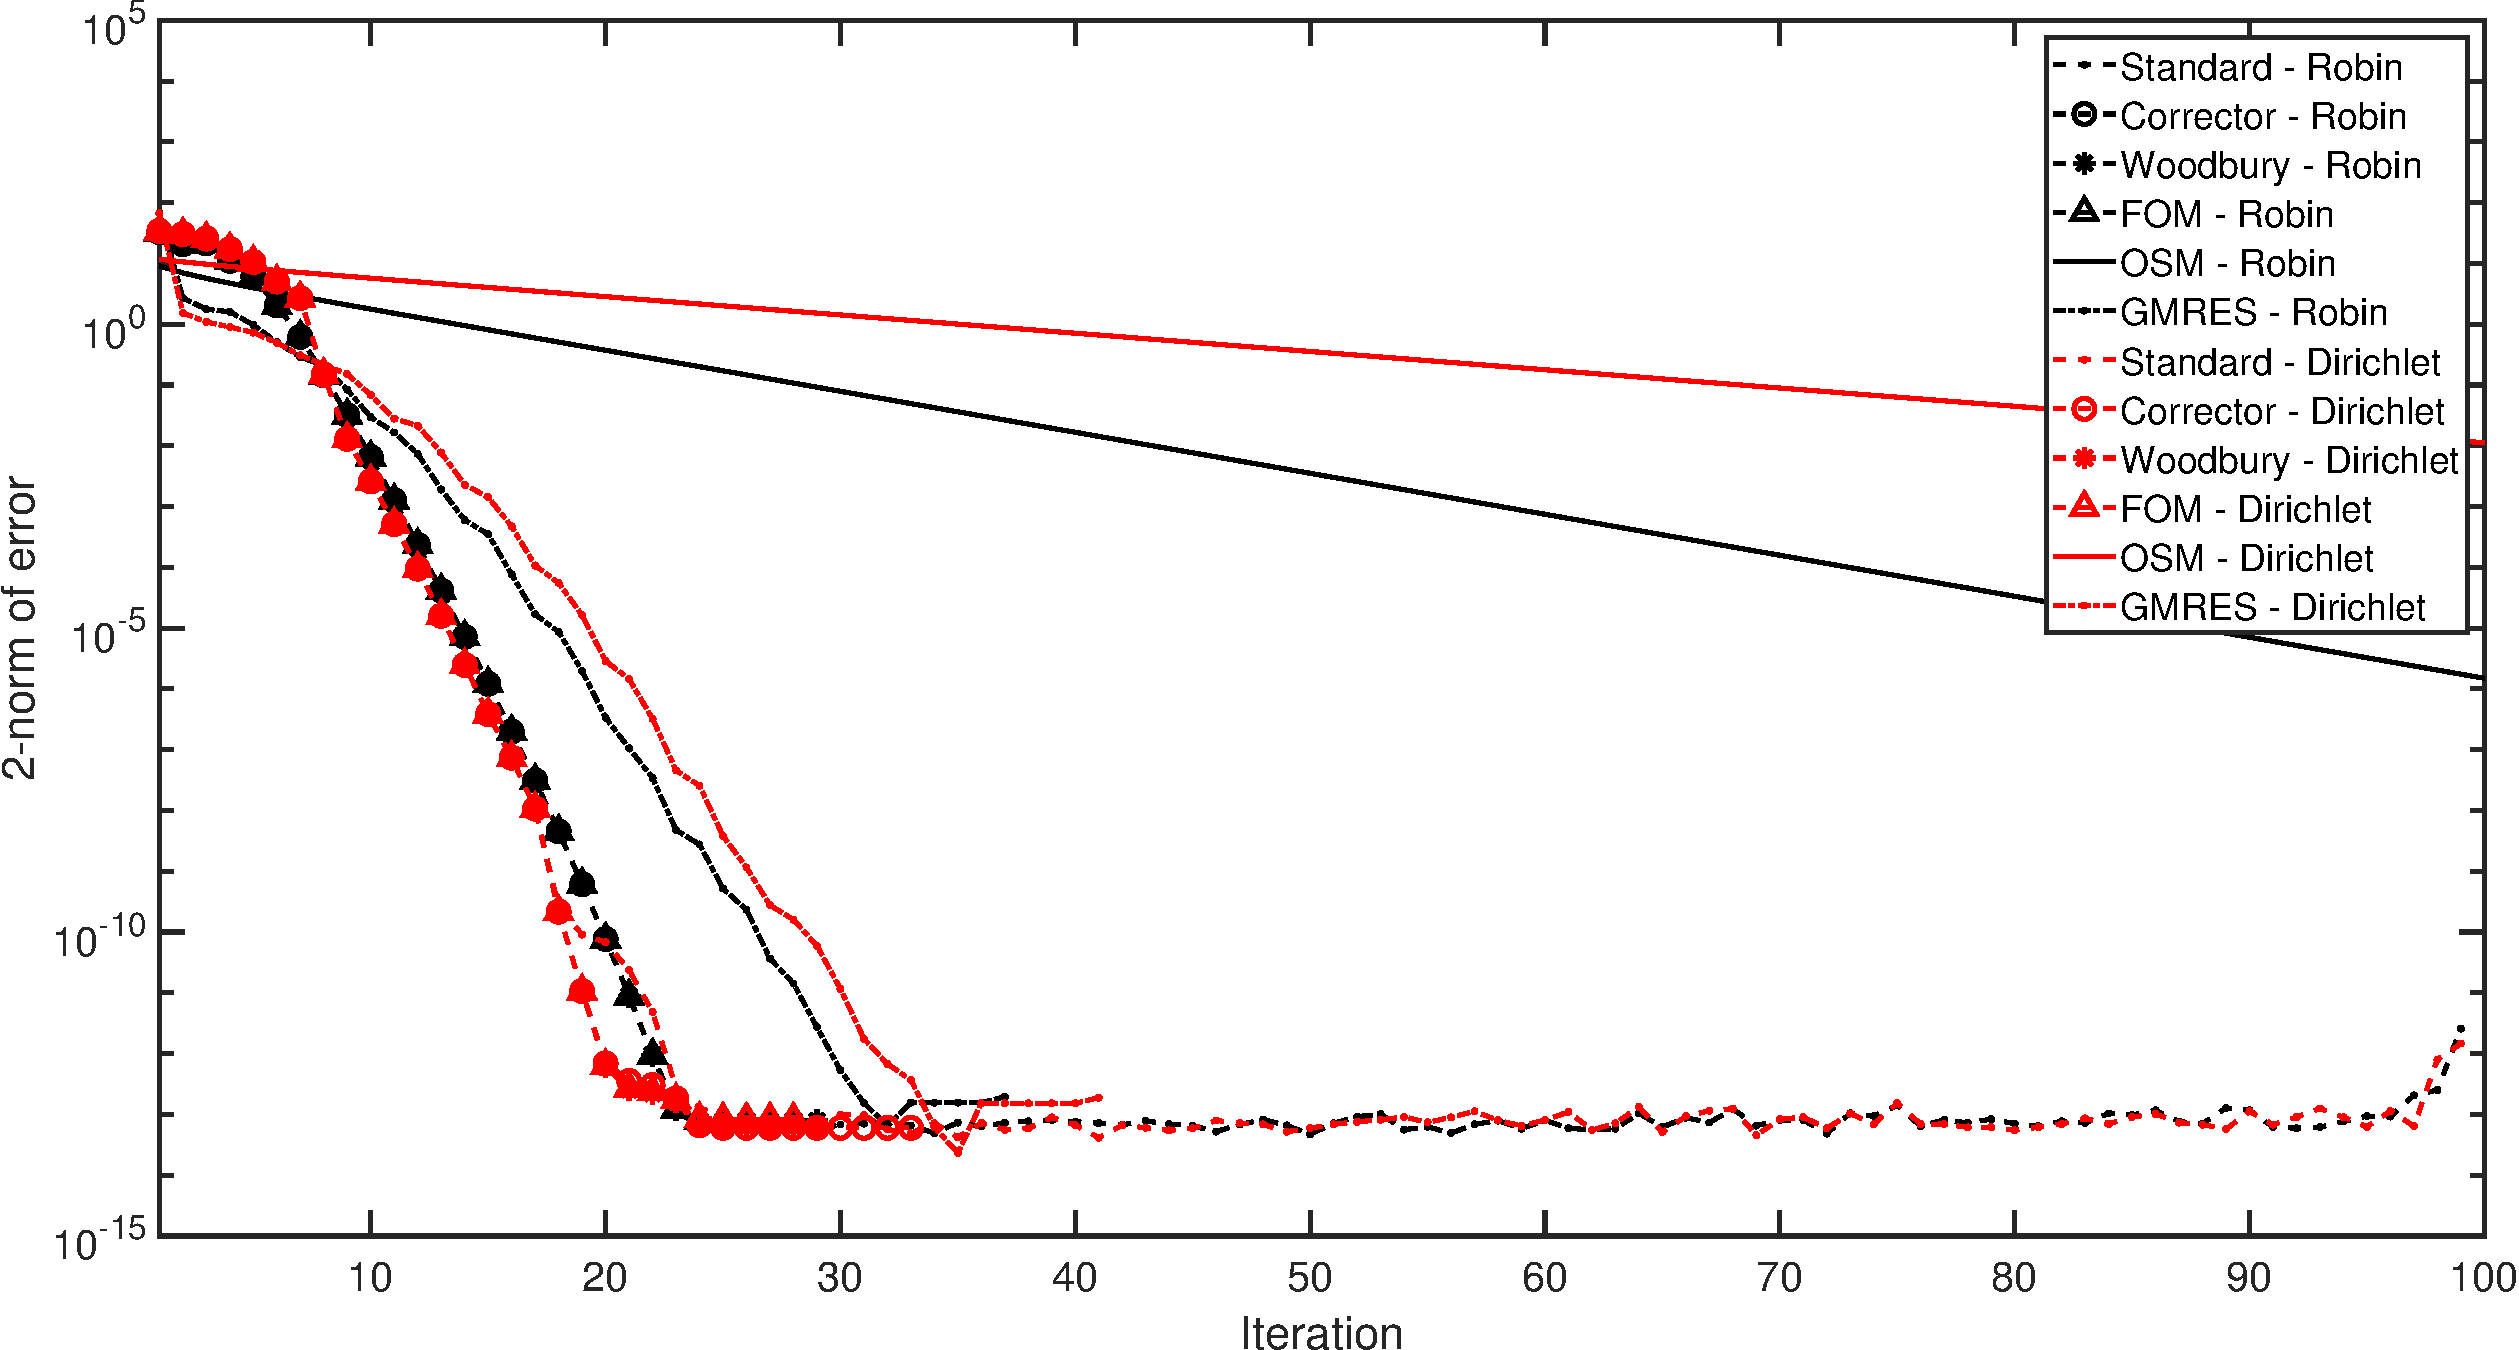
\includegraphics[width=0.75\textwidth]{AOSM/PLOT_fparaAOSMConv_Laplace.pdf}}
%	\caption{Comparison of altAOSM versions in solving equation (\ref{eq: laplace}) with $N=10,000$, $M=100$, using both Robin and Dirichlet boundary conditions.
%	Also shown is the OSM with and without GMRES.}
	\label{fig: compare altAOSM}
	% to update figure: EX_faltAOSMConv_Laplace.m -> h=figure(1); -> exportgraphics(h,'../Figures/PLOT_faltAOSMConv_Laplace.eps');
\end{figure}
\end{frame}

\begin{frame}{Numerical results}
\begin{equation*}
	\begin{cases} u_t(x,y,t) = \Delta u(x,y,t), & (x,y) \in \Omega = [-1,1] \times [-1,1], \ t \in [0,T] \\
		u(x,y,0) = u_0(x,y), & (x,y) \in \Omega, \\
		u(x,y,t) = g(x,y), & (x,y) \in \partial \Omega, \ t \in [0,T]. \end{cases}
\end{equation*}
\begin{figure}
	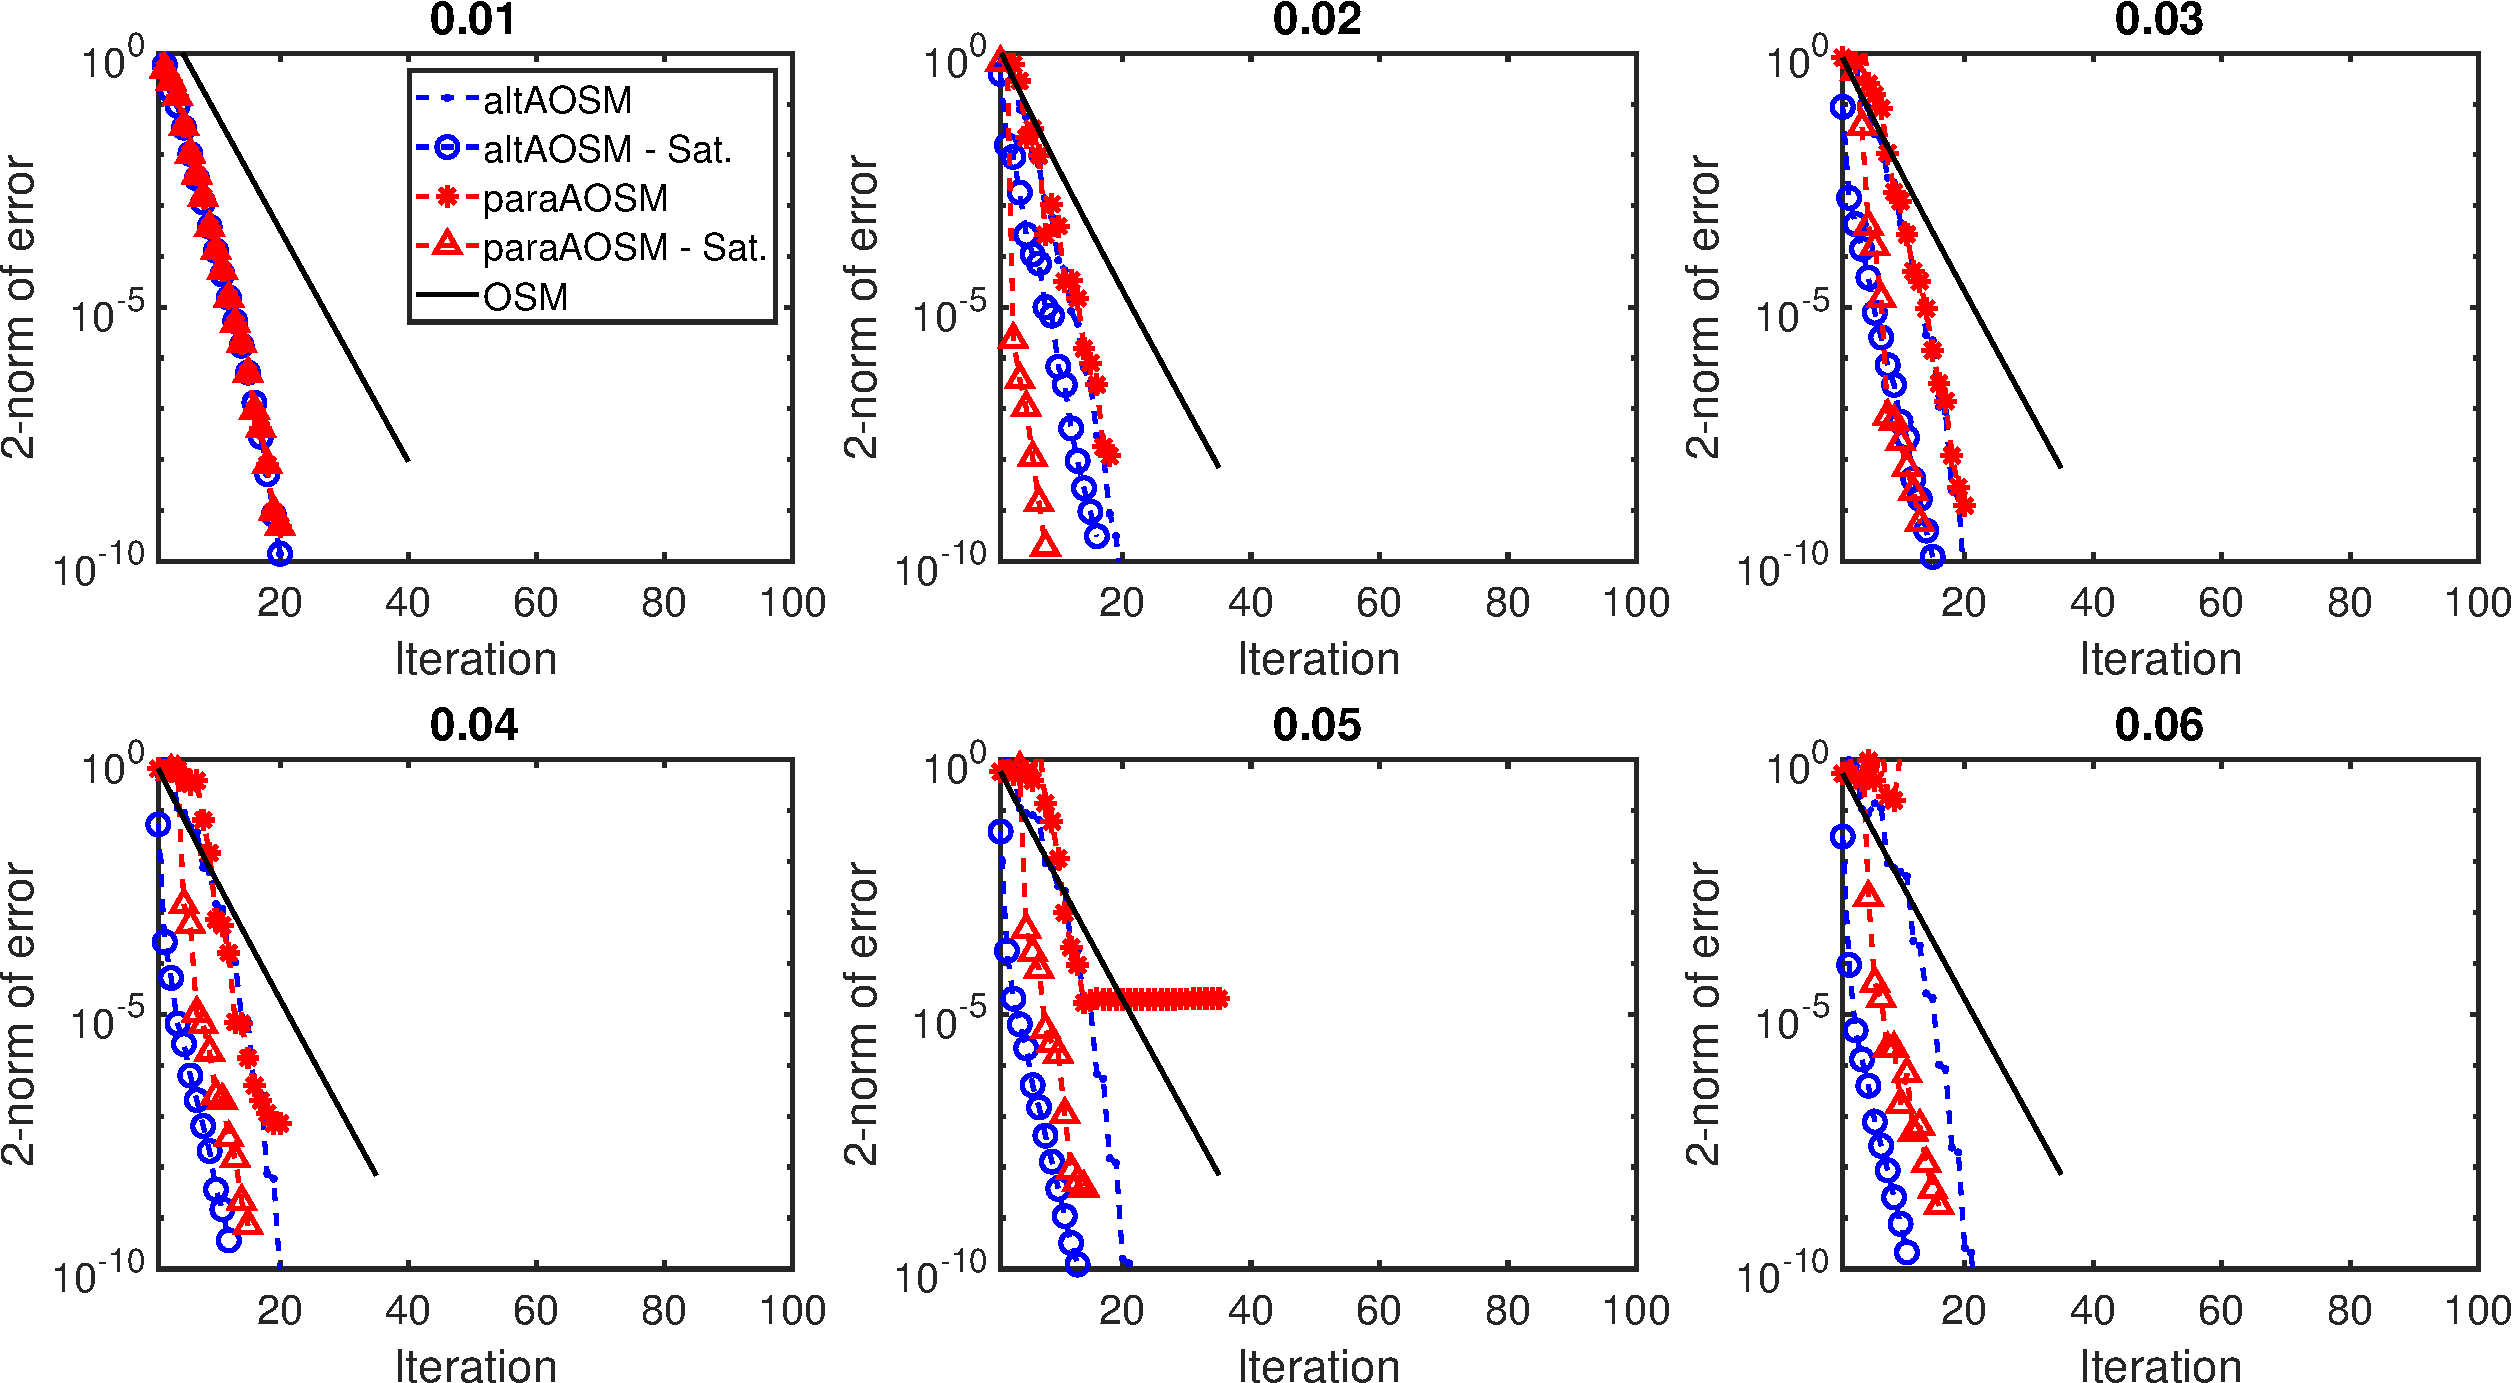
\includegraphics[width=0.75\textwidth]{AOSM/PLOT_AOSMConv_Heat_v1.pdf}
%	\caption{Convergence of OSM and AOSMs at the first six time steps of equation (\ref{eq: discrete heat}).
%		AOSMs that use updated transmission conditions at each time step are labelled `Sat'.}
	\label{fig: heat 1}
	% to update figure: EX_AOSMConv_Heat.m -> h=figure(1); -> exportgraphics(h,'../Figures/PLOT_AOSMConv_Heat_v1.eps');
\end{figure}
\end{frame}

\begin{frame}{Numerical results}
\begin{equation*}
	\begin{cases} -\nabla \left ( \alpha(x,y) \cdot \nabla u(x,y) \right ) = f(x,y), & (x,y) \in \Omega = [0,1] \times [0,1], \\
		u(x,y) = g(x,y), & (x,y) \in \partial \Omega. % = \set{x=-1} \cup \set{x=1} \cup \set{y=-1} \cup \set{y=1} .
	\end{cases}
\end{equation*}
\begin{figure}
	\only<1>{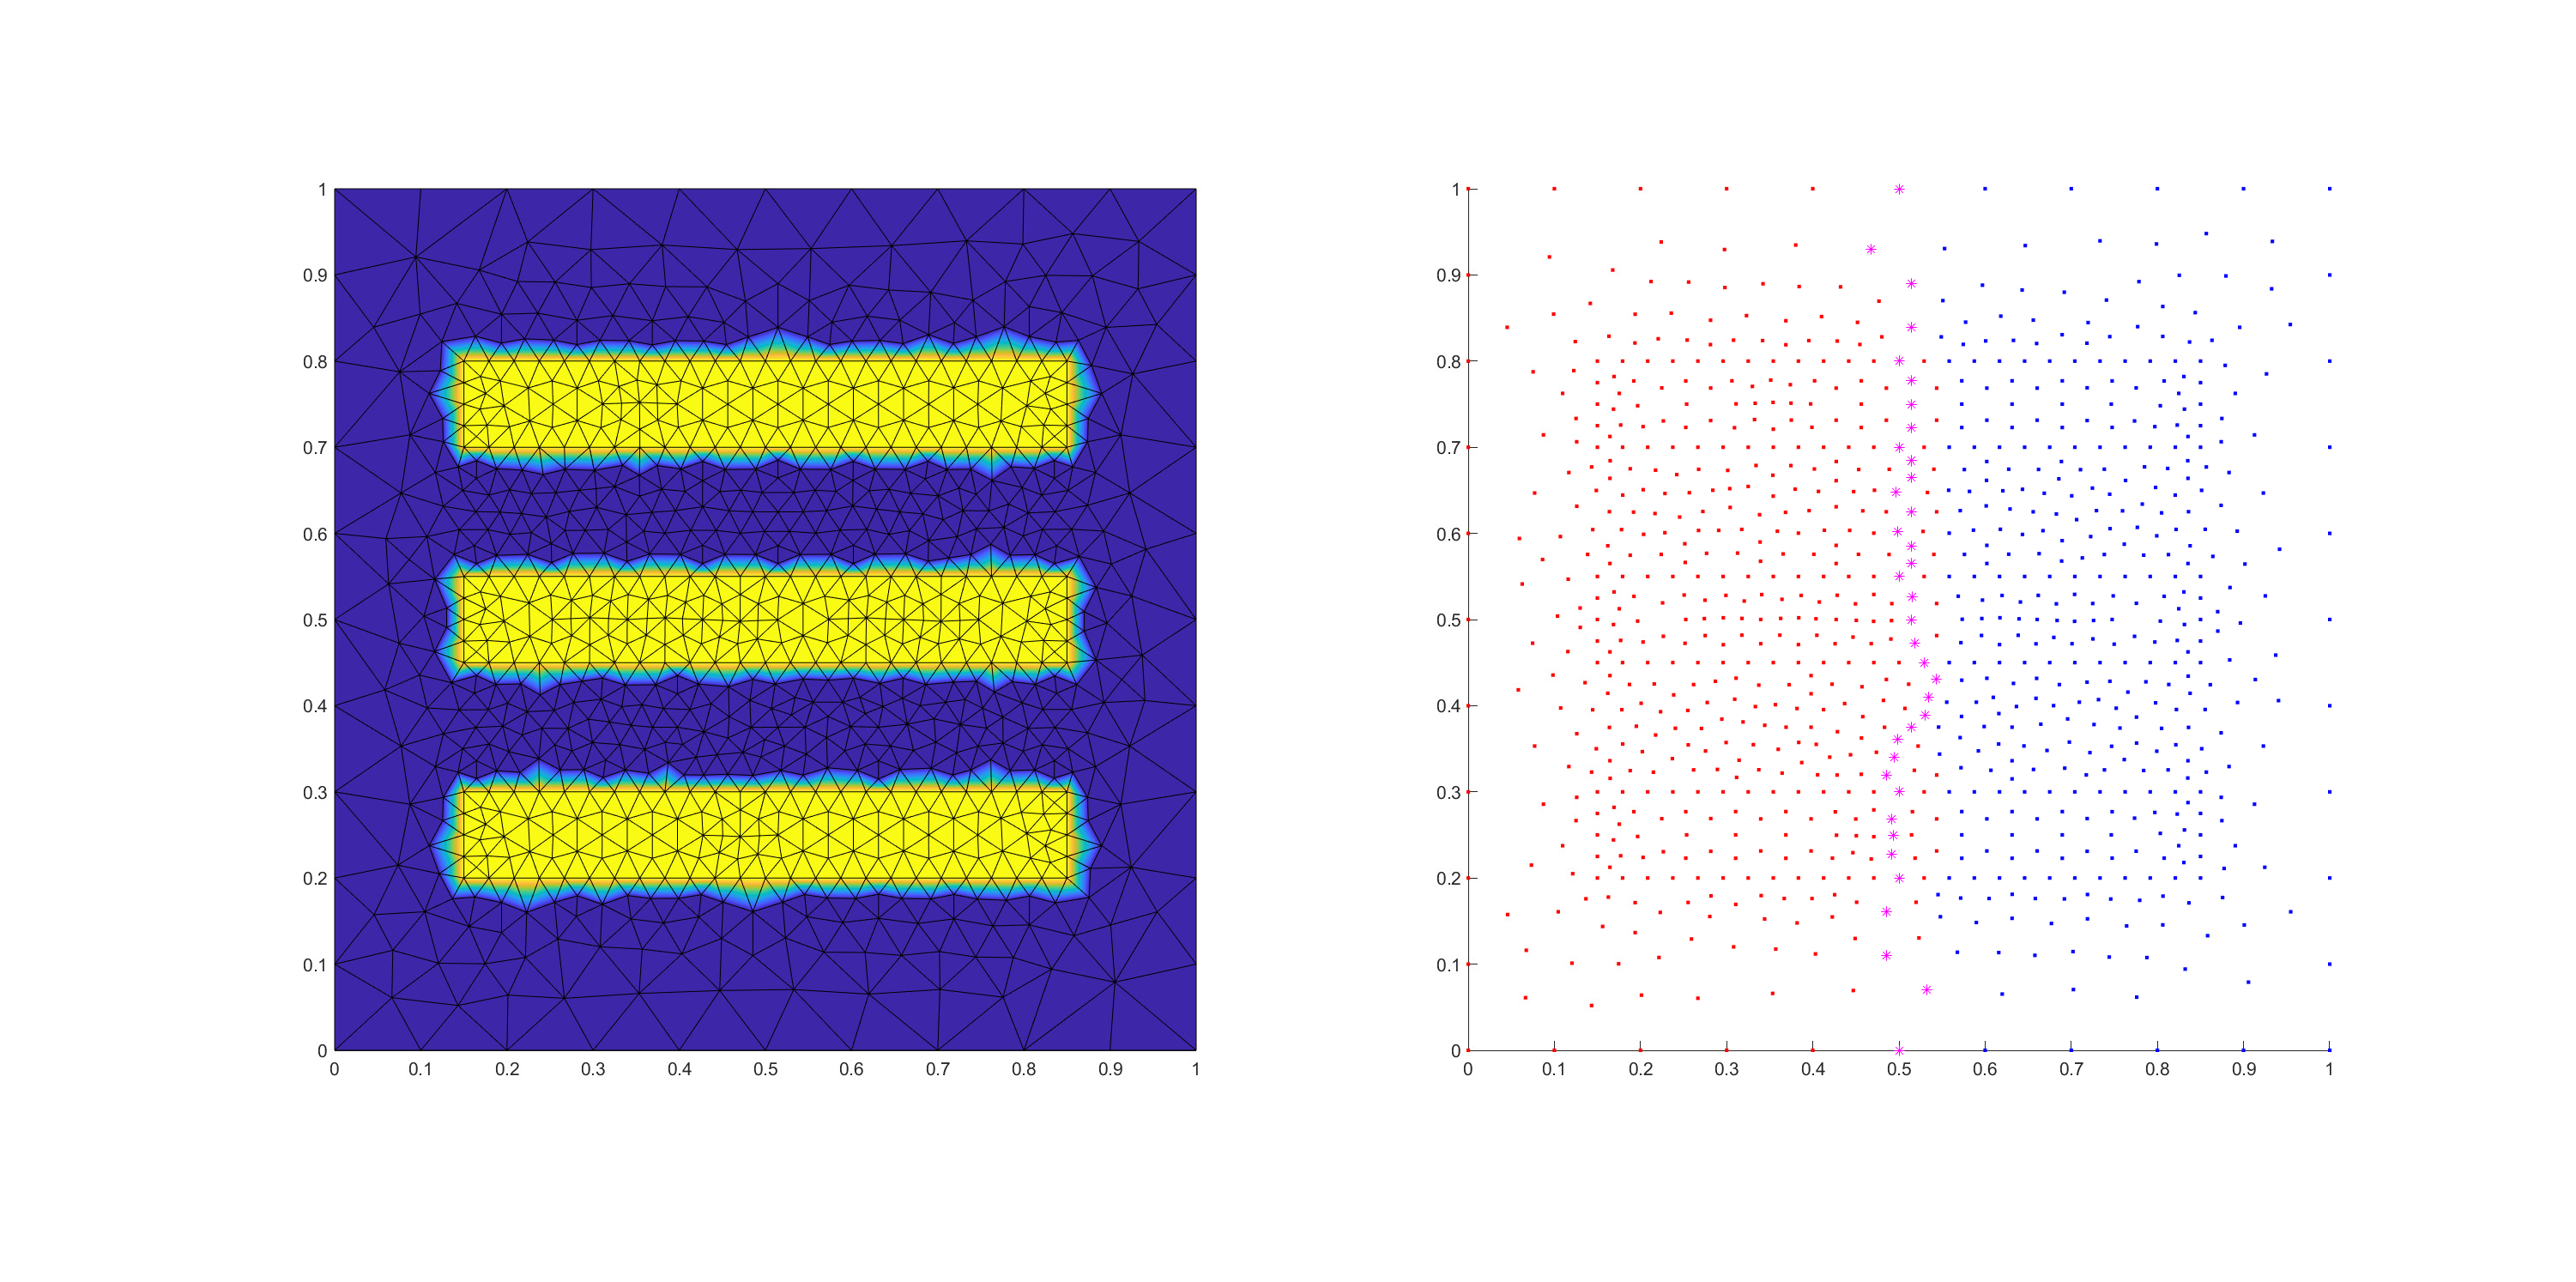
\includegraphics[width=0.75\textwidth]{AOSM/PLOT_MEFPP_loneland_K.pdf}}
	\only<2>{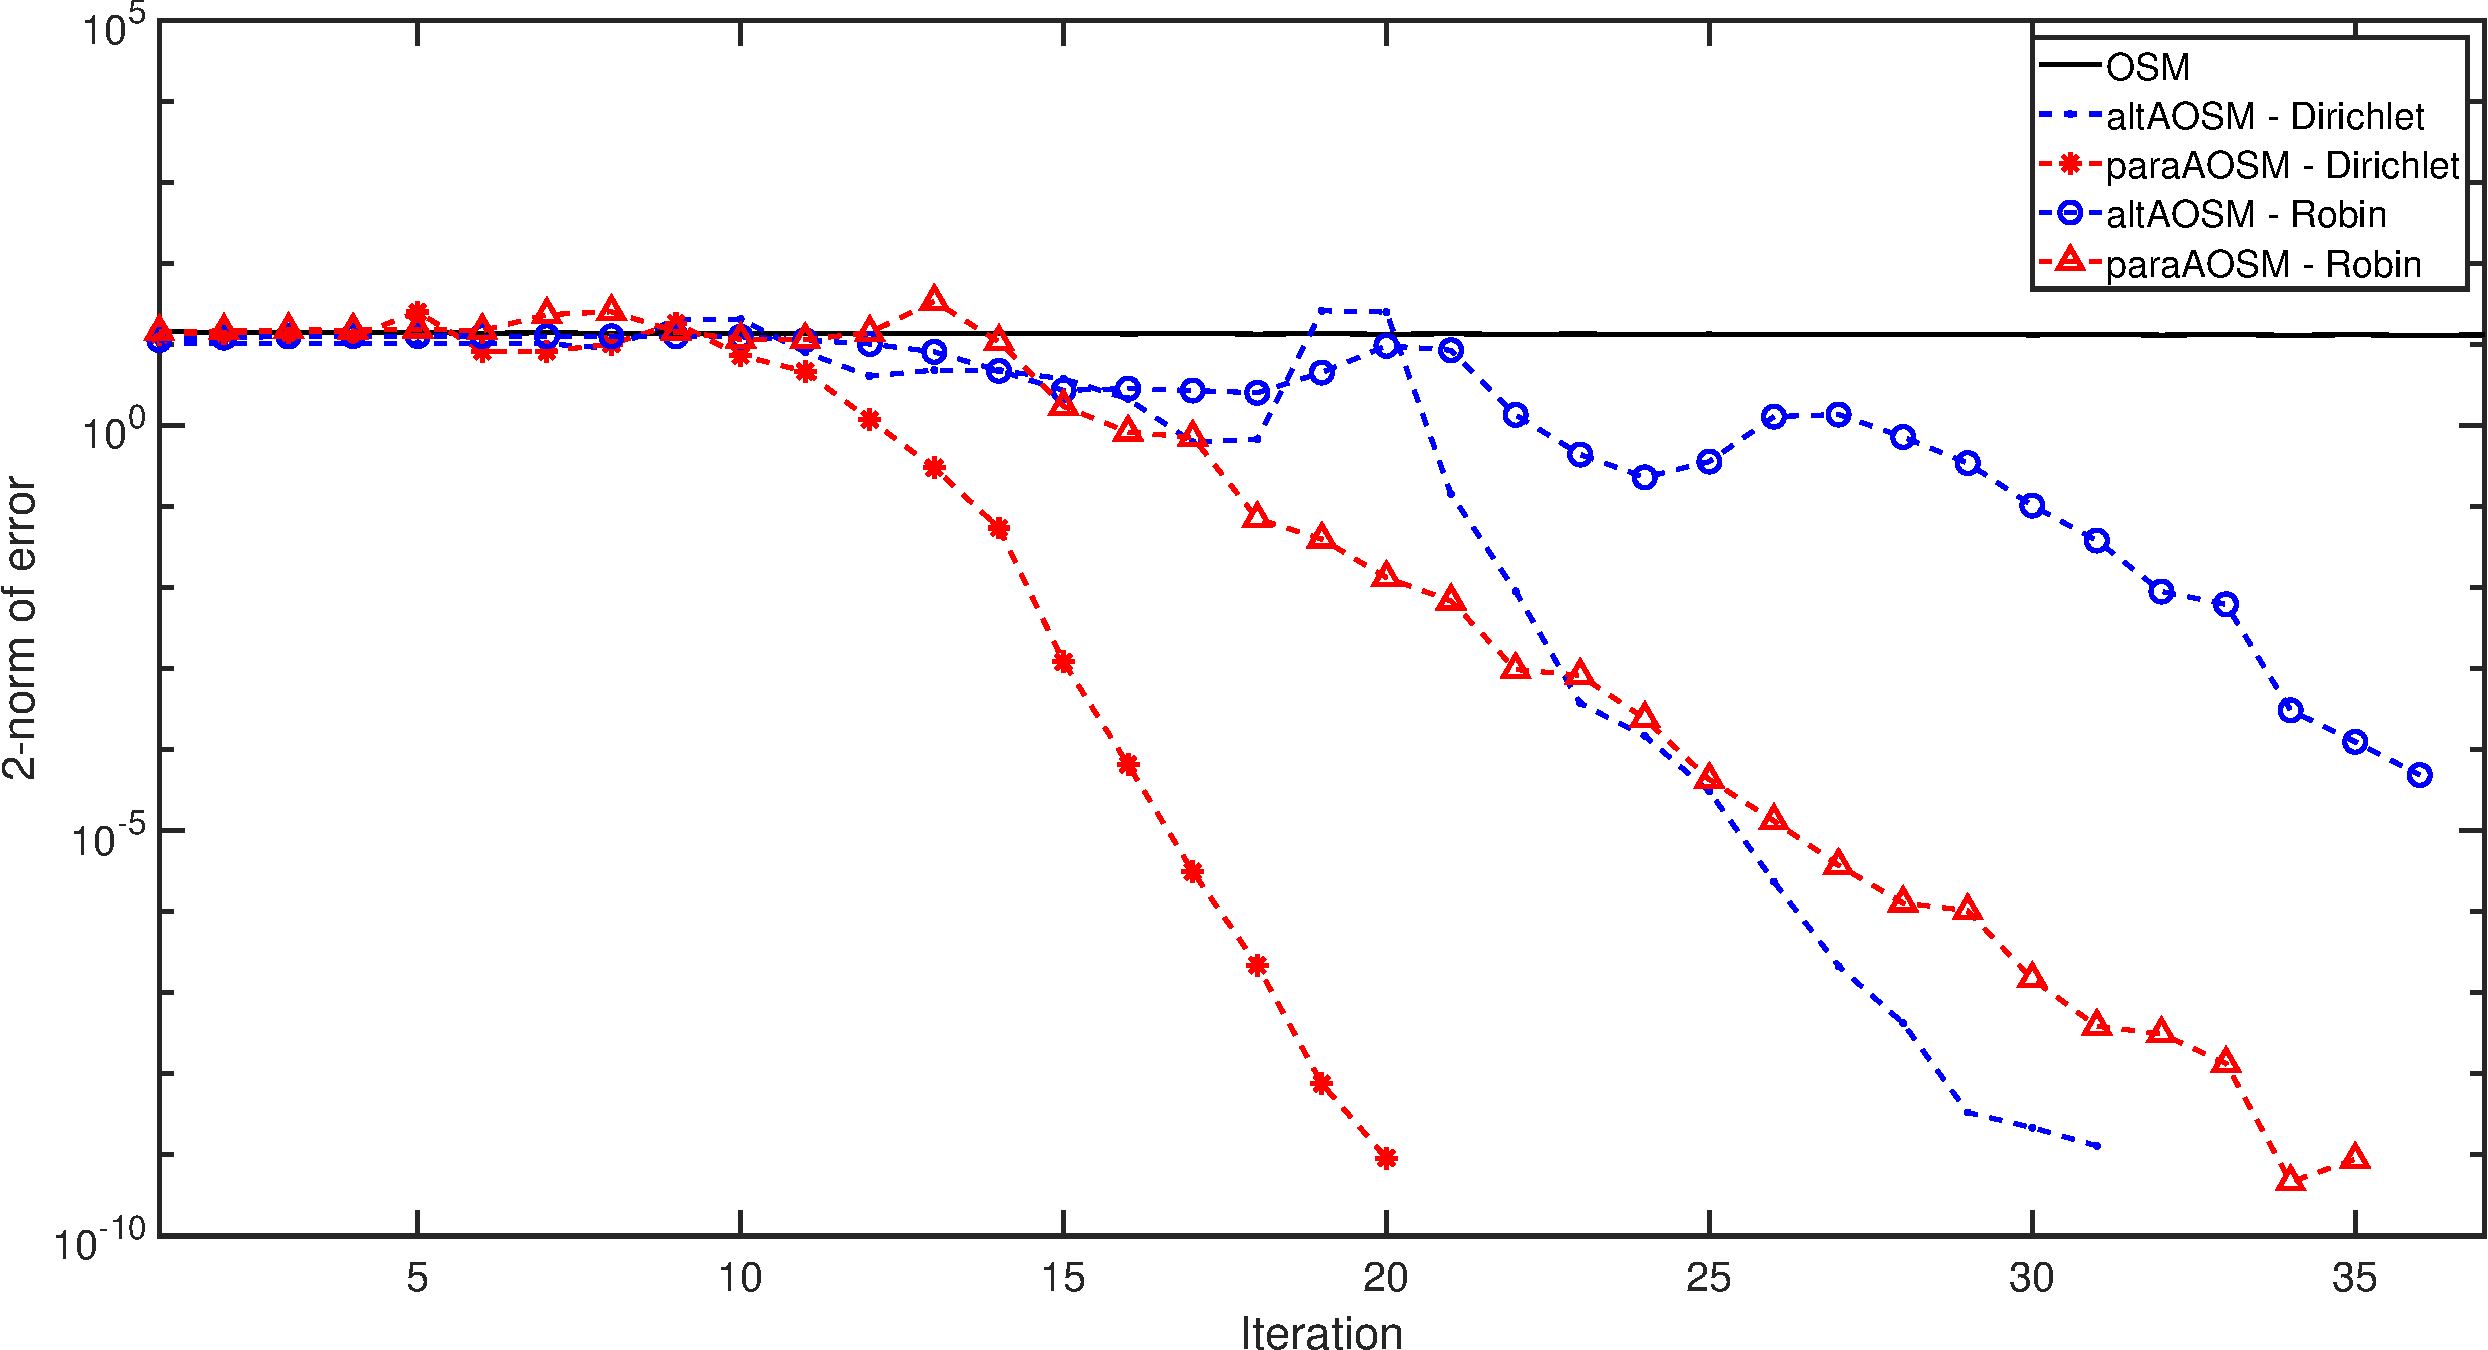
\includegraphics[width=0.75\textwidth]{AOSM/PLOT_MEFPP_loneland_v1.pdf}}
	\only<3>{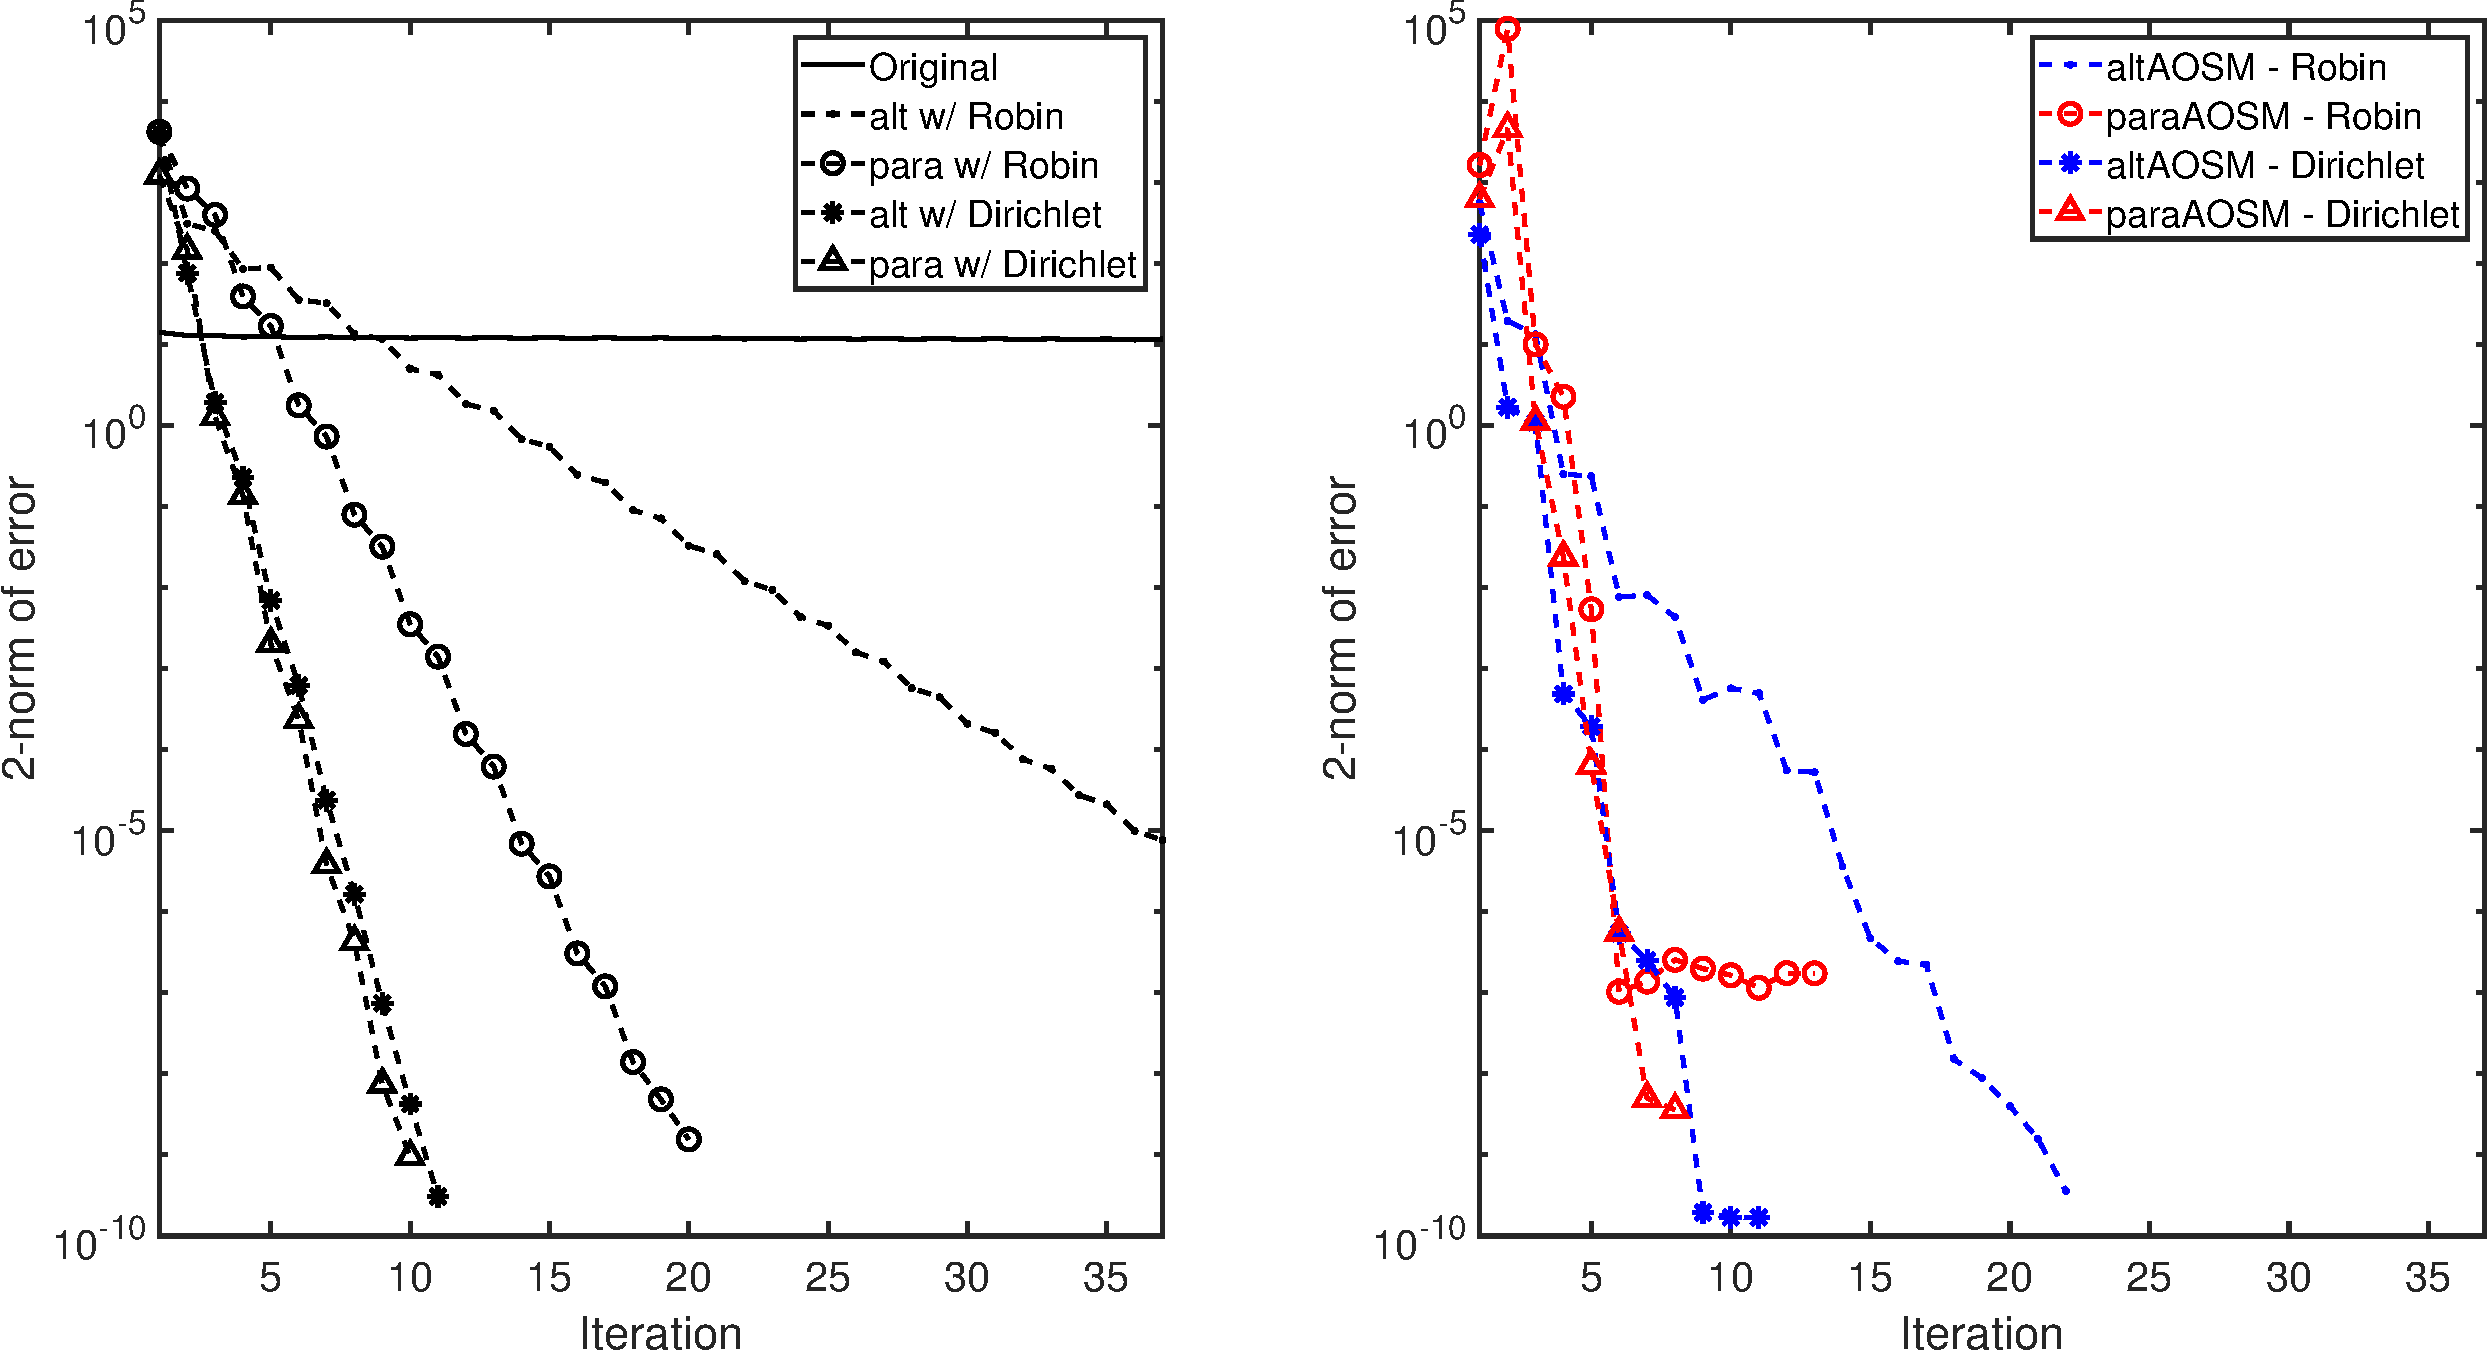
\includegraphics[width=0.75\textwidth]{AOSM/PLOT_MEFPP_loneland_v3.pdf}}
\end{figure}
\end{frame}

\begin{frame}{Conclusions and Future Work}
\begin{itemize}
\item AOSMs give convergence rates comparable to Krylov subspace methods, but without the extra computations.
\item Transmission conditions from AOSMs can be re-used to give fast convergence when repeated solves are required.
\item The paraAOSM has some stability issues that need to be fixed.
\item Nested decompositions will allow more subdomains, but crosspoints need to be resolved for more general decompositions.
\end{itemize}
\end{frame}

\end{document}